%%%%%%%% ICML 2024 EXAMPLE LATEX SUBMISSION FILE %%%%%%%%%%%%%%%%%

\documentclass{article}

% Recommended, but optional, packages for figures and better typesetting:
\usepackage{microtype}
\usepackage{graphicx}
\usepackage{subfigure}
\usepackage{booktabs} % for professional tables


% hyperref makes hyperlinks in the resulting PDF.
% If your build breaks (sometimes temporarily if a hyperlink spans a page)
% please comment out the following usepackage line and replace
% \usepackage{icml2024} with \usepackage[nohyperref]{icml2024} above.
\usepackage{hyperref}


% Attempt to make hyperref and algorithmic work together better:
\newcommand{\theHalgorithm}{\arabic{algorithm}}

% Use the following line for the initial blind version submitted for review:
 \usepackage{icml2024}

% If accepted, instead use the following line for the camera-ready submission:
% \usepackage[accepted]{icml2024}

% For theorems and such
\usepackage{amsmath}
\usepackage{amssymb}
\usepackage{mathtools}
\usepackage{amsthm}

% if you use cleveref..
\usepackage[capitalize,noabbrev]{cleveref}

%%%%%%%%%%%%%%%%%%%%%%%%%%%%%%%%
% THEOREMS
%%%%%%%%%%%%%%%%%%%%%%%%%%%%%%%%
\theoremstyle{plain}
\newtheorem{theorem}{Theorem}[section]
\newtheorem{proposition}[theorem]{Proposition}
\newtheorem{lemma}[theorem]{Lemma}
\newtheorem{corollary}[theorem]{Corollary}
\theoremstyle{definition}
\newtheorem{definition}[theorem]{Definition}
\newtheorem{assumption}[theorem]{Assumption}
\theoremstyle{remark}
\newtheorem{remark}[theorem]{Remark}

% Todonotes is useful during development; simply uncomment the next line
%    and comment out the line below the next line to turn off comments
%\usepackage[disable,textsize=tiny]{todonotes}
\usepackage[textsize=tiny]{todonotes}


% The \icmltitle you define below is probably too long as a header.
% Therefore, a short form for the running title is supplied here:
\icmltitlerunning{Submission and Formatting Instructions for ICML 2024}

\begin{document}

\twocolumn[
\icmltitle{Spurious Sentience:\\
           Dovelating Inflated AI World Model Claims \raisebox{-6pt}{
\includegraphics[scale=0.09]{dove_1f54a-fe0f.png}}}

% It is OKAY to include author information, even for blind
% submissions: the style file will automatically remove it for you
% unless you've provided the [accepted] option to the icml2024
% package.

% List of affiliations: The first argument should be a (short)
% identifier you will use later to specify author affiliations
% Academic affiliations should list Department, University, City, Region, Country
% Industry affiliations should list Company, City, Region, Country

% You can specify symbols, otherwise they are numbered in order.
% Ideally, you should not use this facility. Affiliations will be numbered
% in order of appearance and this is the preferred way.
\icmlsetsymbol{equal}{*}

\begin{icmlauthorlist}
\icmlauthor{Patrick Altmeyer}{yyy}
\icmlauthor{Antony Bartlett}{equal, yyy}
\icmlauthor{Andrew M. Demetriou}{equal, yyy}
\icmlauthor{Cynthia C. S. Liem}{yyy}
\end{icmlauthorlist}

\icmlaffiliation{yyy}{Department of Intelligent Systems, Delft University of Technology, Delft, the Netherlands}

\icmlcorrespondingauthor{Firstname1 Lastname1}{first1.last1@xxx.edu}

% You may provide any keywords that you
% find helpful for describing your paper; these are used to populate
% the "keywords" metadata in the PDF but will not be shown in the document
\icmlkeywords{Machine Learning, Anthropomorphism, Artificial General Intelligence}

\vskip 0.3in
]

% this must go after the closing bracket ] following \twocolumn[ ...

% This command actually creates the footnote in the first column
% listing the affiliations and the copyright notice.
% The command takes one argument, which is text to display at the start of the footnote.
% The \icmlEqualContribution command is standard text for equal contribution.
% Remove it (just {}) if you do not need this facility.

%\printAffiliationsAndNotice{}  % leave blank if no need to mention equal contribution
\printAffiliationsAndNotice{\icmlEqualContribution} % otherwise use the standard text.

\begin{abstract}
This document provides a basic paper template and submission guidelines.
Abstracts must be a single paragraph, ideally between 4--6 sentences long.
Gross violations will trigger corrections at the camera-ready phase.
\end{abstract}

\section{Introduction}
\label{submission}

We humans are prone to seek patterns everywhere. Meaningful patterns have proven useful in helping us make sense of our past, navigate our present and predict the future. Although this tendency to perceive patterns likely leads to evolutionary benefits even when the perceived patterns are false \cite{foster2009evolution}, psychology has revealed a host of situations in which the ability to perceive patterns severely misfires, leading to irrational beliefs in e.g. the power of superstitions \cite{foster2009evolution}, conspiracy theories \cite{van2018connecting}, the paranormal \cite{muller2023linking}, gambler's fallacies \cite{ladouceur1996erroneous} and even interpreting pseudo-profound bullshit as meaningful \cite{walker2019finding}. 

In statistics, misleading patterns are often referred to as spurious relationships: associations, often quantitatively assessed, between two or more variables that are not causally related to each other. Although the formal definition of spuriousness varies somewhat \cite{haig2003spurious}, it distinctly implies that the observation of correlations does not necessarily imply causation. Quantitative data often show non-causal associations (as humorously demonstrated on the \href{http://www.tylervigen.com/spurious-correlations}{Spurious Correlations} website), and as adept as humans are at recognizing patterns, we typically have a much harder time discerning spurious relationships from causal ones. A major contributor is that humans struggle to conceive of actual randomness: e.g. studies show that humans are poor at detecting e.g. \cite{falk1997making}, and creating e.g. \cite{ladouceur1996erroneous} random sequences. A common issue is a lack of expectation that the patterns that hint towards a causal relationship, such as correlations, will still appear at random. This leads even those trained in statistics and probability to perceive illusory correlations, correlations of inflated magnitude (see \cite{nickerson1998confirmation}), or causal relationships in data that is randomly generated \cite{zgraggen2018investigating}.

We argue herein that AI research and development is a perfect storm that encourages our human biases to perceive spurious sparks of general intelligence in AI systems: patterns exhibited by AI systems which are mere reflections of the data used to train them, but that their developers interpret as hints at other, greater cognitive capabilities. In the current race to build the first Artificial General Intelligence (AGI) system, loosely defined as an intelligent system that solve general problems rather than narrow, specific ones, and that demonstrates the abilities of reasoning, planning, and learning from past experience at the level of a human or better e.g. \cite{bubeck2023sparks}, ChatGPT cleared nearly \$1 billion in months of its release according to \href{https://www.bloomberg.com/news/articles/2023-08-30/openai-nears-1-billion-of-annual-sales-as-chatgpt-takes-off}{Bloomberg}, the paid version of which OpenAI claimed only showed 'sparks of AGI'. When combining massive financial incentives with the presence of a challenging and difficult-to-understand technology, that also aims towards human-like problem solving and communication abilities, a situation arises that is fertile for the misinterpretation of spurious cues as hints towards AGI, or other qualities like sentience \footnote{https://www-scientificamerican-com.tudelft.idm.oclc.org/article/google-engineer-claims-ai-chatbot-is-sentient-why-that-matters/} and consciousness.

Present work case studies an example, to which claims of observed AGI 'sparks' in AI research, and reviews work on two human phenomena that are likely to lead to false claims: anthropomorphism, or the attribution of human-like qualities to non-human objects, and confirmation bias, or the seeking-out and/or biased interpretation of evidence in support of one's beliefs. We describe how these phenomena may interact in the context of AI research and development, leading to especially poor inferences about the degree of general intelligence, or lack thereof, within AI systems. We further display results from experiments that at first appear to indicate nascent 'sparks' of AGI, but that stronger tests show are indications of spurious sparks. 

\textcolor{red}{andrew: I'm thinking we can adjust this all to aim towards more 'severe' tests or something. }

%Our society is so invested in finding patterns that today it seems we are more willing than ever to outsource this task to an Artificial Intelligence (AI): an omniscient oracle that leads us down the right path. Unfortunately, history has shown time and again that patterns are double-edged swords: if we attribute the wrong meaning to them, they may lead us nowhere at all, or worse, they may lead us down the dark roads. Despite new and increased momentum in scientific fields concerned with causal inference and discovery, I am also willing to go out on a limb and claim that we are not about to finally reach the top of Judea Pearl’s Causal Ladder through the means of Causal AI.

%I agree with the premise that in a world full of spurious relationships, causal reasoning is our only remedy. But I am very skeptical of claims that AI will magically provide that remedy. This leads me to the title and topic of this post: spurious sentience - patterns exhibited by artificial intelligence that may hint at sentience but are just reflections of the data used to train them. The article is written in response to a recent paper and claims by one of the authors, Max Tegmark, that revealed structure in the latent embeddings of Llama 2 should finally have us believe that LLMs are more than just parrots. Since this is an opinionated post, I feel that I should start with a few disclaimers:

%\begin{itemize}
%    \item I take no issue with the methodological ideas that form the foundation of the article in question: on the contrary, I think that mechanistic interpretability is an interesting and important toolkit that can help us better understand the intrinsics and behavior of opaque artificial intelligence.
%    \item The visualizations are intriguing, the code is open-sourced and the findings are interesting.
%    \item I am surprised that people are surprised by the findings: if we agree that LLMs exhibit strong capabilities that can only be connected to the patterns observed in the data they were trained with, then where exactly do you expect this information to be stored if not in the parameters of the model?\footnote{I would be very surprised—concerned even—if our search for patterns in latent spaces of capable LLMs revealed nothing at all.}
%    \item I therefore do take issue with the way that these findings are being overblown by people with clout. Perhaps the parrot metaphor should not be taken too literally either, but if anything the paper’s findings seem to support the notion that LLMs are remarkably capable of memorizing explicit and implicit knowledge contained in text.
%\end{itemize}

\section{Background}

\subsection{Claims of Artificial General Intelligence}

\textcolor{red}{antony: I will be adding citations and other links later, just getting text down for now.}
As previously mentioned, AGI is the current objective for which the global AI community is shooting for. As observed in 2023, the mainstream implementation of Large Language Models (LLMs) resulted in numerous societal impacts. This enabled those companies with the more mature models to reap considerable monetary returns, despite the numerous negative news feeds. True AGI will be another global milestone for AI and the entire scientific community, thus we already witness massive claims towards it.

Recently, Google DeepMind made claims their AlphaGeometry model \cite{trinh2024geometry} reached a 'milestone' towards AGI. This model has the ability to solve complex geometry problems, which, they state it does without the need for human demonstrations during training. Although this is a fantastic achievement by the team, where we observe the model outperforming previous state of the art (SOTA) models, the underlying model is far from AGI. As discussed in the paper \cite{trinh2024geometry}, AlphaGeometry utilizes a rule-bound deduction engine, allowing the use of an NLP model for further suggestions when it is unable to locate a logical answer. With this combination, it was able to score highly (\textit{25/30} questions solved) where the gold standard human equivalent was \textit{25.9/30}.

However, as noted by Hector Zenil \cite{hector2024linkedin}, that work such as this had been initially introduced in the 1950s. Without the use of an LLM, logical inference systems proved 100\% accurate in proving all the theorems of Euclidean Geometry. They were able to achieve this success due to geometry being an axiomatically closed system. Therefore, despite DeepMinds success in creating a powerfully fast Geometry solving machine, it is still far from being an AGI.

One of the more contentious pieces of literature recently studied is the paper by \cite{gurnee2023language}. This paper, which was the inspiration for our work, received numerous points of critical feedback when they discussed their work on the X\footnote{https://twitter.com} (formally Twitter) platform. Although not directly mentioning AGI, they do hint at the emergence of intelligence, specifically with the creation of the world model.

They claim said models generate an internal representation of the world, with which spatiotemporal representations are created. Further to this we see claim to the generalization of tasks, in which the model can answer questions regarding spatial and temporal relationships, without the need for further training. Although these can be seen as building blocks for a more comprehensive model, it is also fair to assume that it is mere conjecture and more likely spurious correlations.

As we also consider the paper by the Microsoft Research team \cite{}, despite the illusion of a claim that GPT-4 shows sparks of AGI, they do not directly claim that GPT-4 has AGI. However they do claim that we are moving closer to this goal, which is not an outlandish claim given the advancements we have seen with AI in recent years.

\subsection{Confirmation Bias}

Confirmation bias is generally defined as favoring interpretations of evidence that support existing beliefs or hypotheses \cite{nickerson1998confirmation}. Importantly, it need not be fully conscious. Rather, theory suggests that it is a category of implicit and unconscious processes that involve assembling one-sided evidence, and shaping it to fit one's belief. Equally importantly, is that theory suggests these behaviors may be motivated or unmotivated: one may selectively seek, attend to, or interpret evidence in favor of a hypothesis for which they may or may not have a personal interest in supporting. 

Hypotheses in computer science fields related to AI are often implicit. Often framed as informally that a given system is more accurate or efficient compared to other systems, and not typically articulated as they are in other fields, with specific conditions and in some instances numerical values or effect sizes assigned to each competing hypothesis. However with regards to claims that outputs of a system hint towards emerging qualities like AGI, hypotheses necessarily become more explicit: either one interprets outputs as in support of hints towards AGI (the competing hypothesis), or as merely the result of an algorithm integrating qualities from the data it was trained on (the null hypothesis). 

Confirmation bias in hypothesis testing may manifest as a number of behaviors, as \cite{nickerson1998confirmation} reviews. Scientists may pay little to no attention to competing hypotheses or explanations, e.g. only considering the likelihood that outputs of system support one's claims, and not the likelihood that the same outputs might occur if one's hypothesis is false. Similarly, bias may show when failing to articulate a sufficiently strong null hypothesis leading to a 'weak' or 'non-risky' experiment, a problem articulated in response to a number of scientific crises \cite{claesen2022severity}. In extreme cases, propositions may be made that cannot be falsified based on how they are formulated. If the threshold to accept a favored hypothesis is too low, observations consistent with the hypothesis are almost guaranteed, and in turn fail to severely test the claim in question. Thus, one is far more likely to show evidence in favor of their beliefs by posing a weak null hypotheses. Related to the formulation of hypotheses is the interpretation of evidence in favor of competing hypotheses, wherein people will interpret identical evidence differently based on their beliefs. As \cite{nickerson1998confirmation} reviews, individuals may place greater emphasis or milder criticism on evidence in support of their hypothesis, and lesser emphasis and greater criticism on evidence that opposes it. 



\subsection{Anthropomorphism}

Research on anthropomorphism has repeatedly shown the human tendency to attribute human-like characteristics to non-human agents and/or objects. These might include the weather and other natural forces, pets and other animals, and gadgets and other pieces of technology \cite{epley2007seeing}. Formally studied as early as 1944, \cite{heider1944experimental} observed that humans can correctly interpret a narrative whose characters are abstract 2D shapes, but also that humans interpreted random movements of these shapes as having a human-like narrative. Anthropomorphism was implied because the descriptions of the 2D shapes went beyond their observable movements, and included representations of mental, emotional, and cognitive processes that resemble humans, findings that have been expanded upon substantially in the following decades (see \cite{epley2007seeing} for review). 
Relevant to AI and the degree to which it resembles AGI, anthropomorphizing may occur independently of whether such judgments are accurate, and as a matter of degree: at the weaker end, one may employ anthropomorphism as a metaphorical way of thinking or explaining, and at the stronger end may attribute human emotions, cognition, and intelligence to AI systems. As \cite{epley2007seeing} note, literature has shown that even weak metaphorical anthropomorphism may affect how humans behave towards non-human agents.

Modern theory of anthropomorphism suggests there are three key components, one of which is a cognitive feature, and two of which are motivations. The first involves the easy availability of our experiences as heuristics that can be used to explain external phenomena: "...knowledge about humans in general, or self-knowledge more specifically, functions as the known and often readily accessible base for induction about the properties of unknown agents" (p.866) \cite{epley2007seeing, waytz2010social}. Thus, our experience as humans is an always-readily-available template to interpret the world, including non-human agent behaviors. This may be more so when the behaviors of that agent are made to resemble humans, which can be a benefit to the second key component of the theory: a motivational state to anthropomorphize among individuals experiencing loneliness, social isolation, or otherwise seeking social connection \cite{epley2007seeing, waytz2010social}. An illustration is the example of Tom Hank's character in the film Castaway who has conversations with a ball he calls "Wilson". Those experiencing a need for social connection may begin to imbue objects, gadgets, pets etc. with human-like qualities to satisfy their social needs, anticipating the now-forming market for apps and robots to fill this function \cite{salles2020anthropomorphism}. 

The motivation as a human to be competent, so-called effectance motivation, is the most relevant to this discussion, as it describes the need to effectively interact with our environments, including the technologies of the day \cite{epley2007seeing}. When confronted with an opaque technology, a person may interpret its behaviors using the most readily available template at hand, namely their personal human experience, in order to facilitate learning \cite{epley2007seeing, waytz2010social}. Perceiving human characteristics, motivations, emotions, and cognitive processes from one's own experiences in a technology e.g. an AI chatbot, allows for a ready template of comparison at the very least, and possibly an increase in ability to make sense of, and even predict, the agents behaviors. This may include being placed in a position to master a certain technology, whether by incentives to learn, or fear of poor outcomes should one not manage to learn. One such situation is the increasing demand for 'AI' skills among AI non-experts: e.g. job postings for individuals with skills in 'GenAI' have increased dramatically since the release of ChatGPT\footnote{Retrieved 19/01/2023 from https://lightcast.io/resources/blog/generative-ai-10-19-2023}, and individuals who are in a position to adopt to the technology are projected to benefit \footnote{Retrieved 19/01/23 from https://www.imf.org/en/Publications/Staff-Discussion-Notes/Issues/2024/01/14/Gen-AI-Artificial-Intelligence-and-the-Future-of-Work-542379}. Thus, individuals in advanced economies may experience a pressure to rapidly learn how to effectively use and understand an opaque technology that appears to behave human-like in at least some ways, and by imbuing the technology with humanity may in turn ease their learning curve. 

These pressures extend to experts as well, in both scholarly and commercial fields. Academics face considerable pressures to publish work in the field of AI: citation metrics and scholarly publications remain the primary metric for tenure and promotion e.g. \cite{alperin2019significant}, and the number of publications in the AI field has boomed as evidenced in overall scholarly publications \footnote{ Retrieved 23/01/23 from https://ourworldindata.org/grapher/annual-scholarly-publications-on-artificial-intelligence?time=2010..2021 }, and in peer-reviewed publications \cite{Maslej2023-pi}, with both more than doubling from 2010 to 2020. The adoption of techniques underlying technologies with the AI label, i.e. machine learning, has spread to fields far beyond Computer Science, e.g. Astronomy and Physics to Medicine and Psychology\footnote{Retrieved 23/01/23 using the search string "TITLE-ABS-KEY ( ( machine  AND  learning )  OR  ( artificial  AND  intelligence )  OR  ai )  AND  PUBYEAR  >  2009  AND  PUBYEAR  <  2024 " from the \href{https://www.scopus.com/}{SCOPUS} database}. Outside of academia, the number of jobs requiring AI expertise have increased several fold, with demand for 'Machine Learning' skills clusters having increased over 500\% from 2010 to 2020 \cite{Maslej2023-pi}. Given the strong incentives to be AI-competent, it is perhaps not surprising to see human-metaphors in how AI has been designed and described, even though these very designs prevent it from ever having the cognitive functions of a human e.g. \cite{salles2020anthropomorphism, van2023reclaiming}. 

\section{Patterns in Latent Spaces and How to Find
Them}\label{patterns-in-latent-spaces-and-how-to-find-them}

To support our claim that observing patterns in latent spaces should not generally surprise us, we will now go through a couple of simple examples. To illustrate further that this phenomenon is neither surprising nor unique to the field of computer science, we will borrow draw on ideas from the fields of Economics and Finance in this section. We will start with very simple examples to demonstrate that even small and simple models can learn meaningful representations of the data. The final example in Section \ref{ex-llm} is a bit more involved and closer in spirit to the experiments conducted by \citet{gurnee2023language}. As we go along, we will try to discuss both the benefits and potential pitfalls of finding patterns in latent spaces.

\subsection{Example: Random Projections of World Models}\label{example-deep-learning}

The Llama-2 model has ingested huge amounts of publicly available data from the internet including Wikipedia dumps from the June-August 2022 period \citep{touvron2023llama}. It is therefore highly likely that the training data contains geographical coordinates, either directly or indirectly. At the very least, we should expect that the model has seen features during training that are highly correlated with geographical coordinates. The model itself is essentially a very large latent space to which all features are randomly projected in the very first instance, before being passed through a series of layers which are gradually trained for downstream tasks.

In our first example in this section, we simulate this scenario, stopping short of training the model. In particular, we

\begin{itemize}
\tightlist
\item
  Take the
  \href{https://github.com/wesg52/world-models/blob/main/data/entity_datasets/world_place.csv}{world\_place.csv}
  that was used in \cite{gurnee2023language}, which maps locations/areas
  to their latitude and longitude. For each place, it also indicates the
  corresponding country.
\item
  Take the subset that contains countries that are currently part of the
  top 10
  \href{https://www.fifa.com/fifa-world-ranking/men?dateId=id14142}{FIFA
  world ranking}.
\item
  Assign the current rank to each country, i.e.~Argentina gets 1, France
  gets 2, \ldots{}
\item
  Transform the longitude and latitude data, respectively, as follows:
  \(\rho \cdot \text{coord} + (1-\rho) \cdot \epsilon\) where
  \(\rho=0.5\) and \(\epsilon \sim \mathcal{N}(0, 5)\). This is to
  ensure that the training data only involves a noisy version of the
  coordinates.
\item
  Next, encode all features except the FIFA world rank indicator as
  continuous variables: \(X^{(n \times m)}\) where \(n\) is the number
  of samples and \(m\) is the number of resulting features.
\item
  Additionally, add a large number of random features to \(X\) to
  simulate the fact that not all features ingested by Llama-2 are
  necessarily correlated with geographical coordinates. Let \(d\) denote
  the final number of features, i.e.~\(d=m+k\) where \(k\) is the number
  of random features.
\item
  Initialize a small neural network, let's call it a \emph{projector},
  that maps from \(X\) to a single hidden layer with \(h<d\) hidden
  units and sigmoid activation and then from there to a
  lower-dimensional output space.
\item
  Without performing any training on the \emph{projector}, we simply
  compute a forward pass of \(X\) through the \emph{projector} and
  retrieve the activations \(\mathbf{Z}^{(n\times h)}\).
\item
  Next, we perform the linear probe on \(\mathbf{Z}\) through Ridge
  regression:
  \(\mathbf{W} = (\mathbf{Z}'\mathbf{Z} + \lambda \mathbf{I}) (\mathbf{Z}'\mathbf{Y})^{-1}\)
  where \(\mathbf{Y}\) is the \((n \times 2)\) matrix containing the
  longitude and latitude for each sample.
\item
  Finally, we compute the predicted coordinates for each samples as
  \(\widehat{\mathbf{Y}}=\mathbf{Z}\mathbf{W}\) and plot the results on
  a world map (see Figure~\ref{fig-map}).
\end{itemize}

\begin{figure}

{\centering 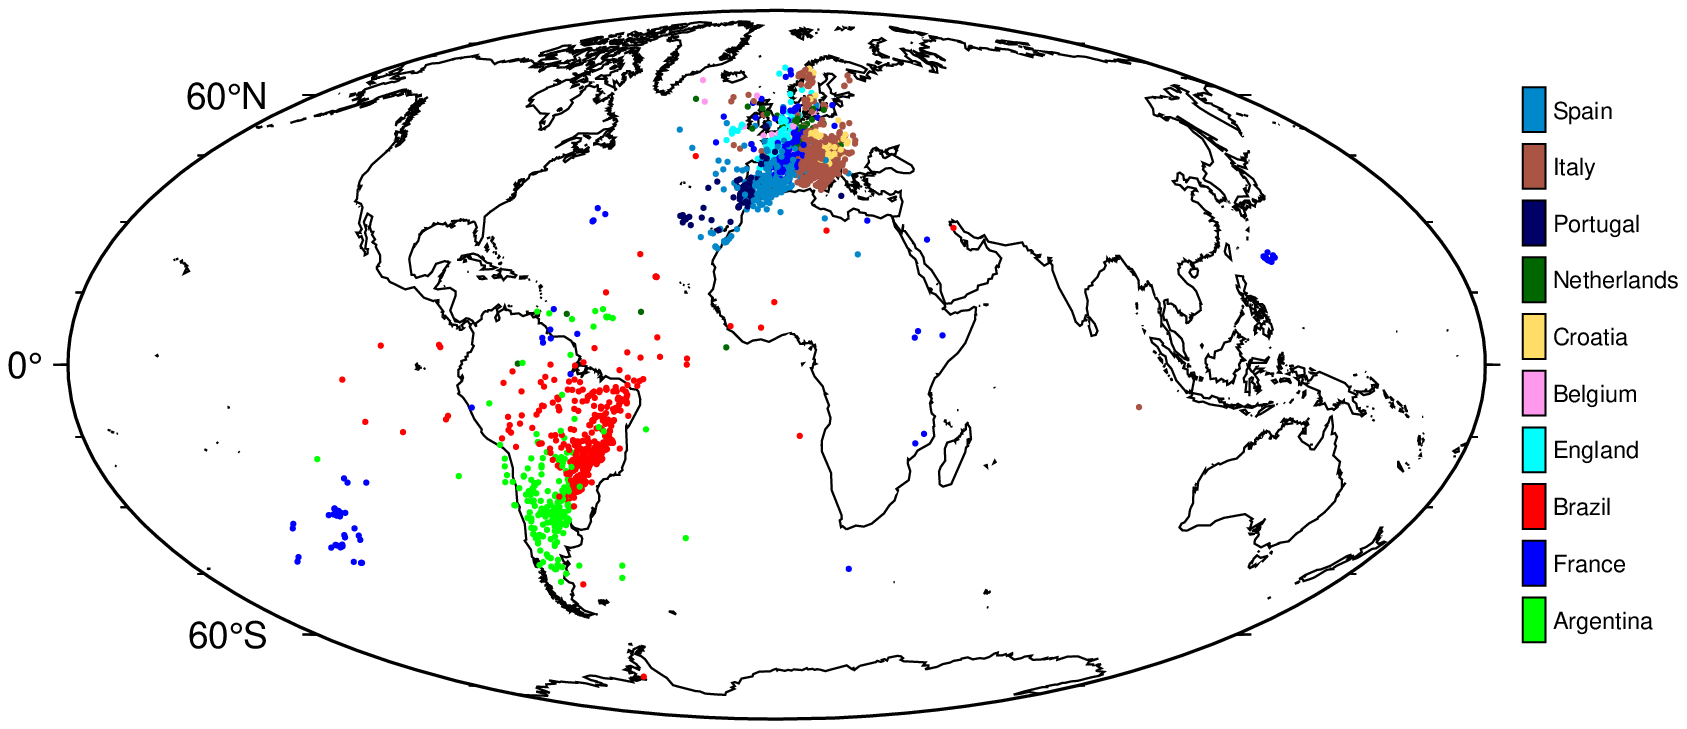
\includegraphics[width=0.5\textwidth]{results/figures/map.png}

}

\caption{\label{fig-map}Predicted coordinate values (in-sample) from a linear probe on final-layer activations of an untrained neural network.}

\end{figure}

While this is admittedly a somewhat contrived example, it serves to illustrate the point that if we randomly project a small number of features that are highly correlated or predictive of the target into a large enough space, we should expect to be able to recover meaningful representations of the target from the latent space. Similarly, \cite{alain2018understanding} observe that even before training a convolutional neural network on MNIST data, the layer-wise activations can already be used to perform binary classification. In fact, it is well-known that random projections can be used for prediction tasks \cite{dasgupta2013experiments}.

\subsection{Example: Principal Component
Analysis}\label{example-principal-component-analysis}

For our next example, we will move beyond randomness and illustrate how principal component analysis can be used to recover meaningful and compact latent representations from data in an unsupervised manner. 

The yield curve is a popular tool for investors and economists to gauge the health of the economy. It plots the yields of bonds against their maturities. The slope of the yield curve is often used as a predictor of future economic activity: a steep yield curve is associated with a growing economy, while a flat or inverted yield curve is associated with a contracting economy.

Of course, US Treasuries are not the only bonds that are traded in the market. To get a more complete picture of the economy, analysts might
therefore be interested in looking at the yield curves of other bonds as
well. In particular, we might be interested in predicting economic
growth based on the yield curves of many different bonds. The problem
with that idea is that it is cursed by high dimensionality: we would end
up modelling a single variable of interest (economic growth) with a
large number of predictors (the yields of many different bonds). To deal
with the curse of high dimensionality it can be useful to decompose the
yield curves into sets of principal components.

To compute the principal components we can decompose the matrix of yields \(\mathbf{Y}\) into a product of its singular vectors and values: \(\mathbf{Y}=\mathbf{U}\Sigma\mathbf{V}^{\prime}\). To put this into the broader context of the article, however, let us simply refer to \(\mathbf{U}\), \(\Sigma\) and \(\mathbf{V}^{\prime}\) as latent embeddings of the yield curve (they are latent because they are not directly observable).

The top panel in Figure~\ref{fig-pca} shows the first two principal
components of the yield curves of US Treasury bonds over time. Vertical
stalks indicate the key dates during the onset and aftermath of the
crisis, which we discussed above. For both components, we can observe
some marked shifts between the two dates - but can we attribute any
meaning to these shifts? It turns out we can: for comparison, the bottom
panel in Figure~\ref{fig-pca} shows the average level and spread of the
yield curves over time. The first principal component is strongly
correlated with the level of the yield curve, while the second principal
component is strongly correlated with the spread of the yield curve. To
put it in AI-lingo:

\begin{quote}
The estimated latent embeddings of the yield curve are characterized by
patterns observed in the data.
\end{quote}

\begin{figure*}

\centering{

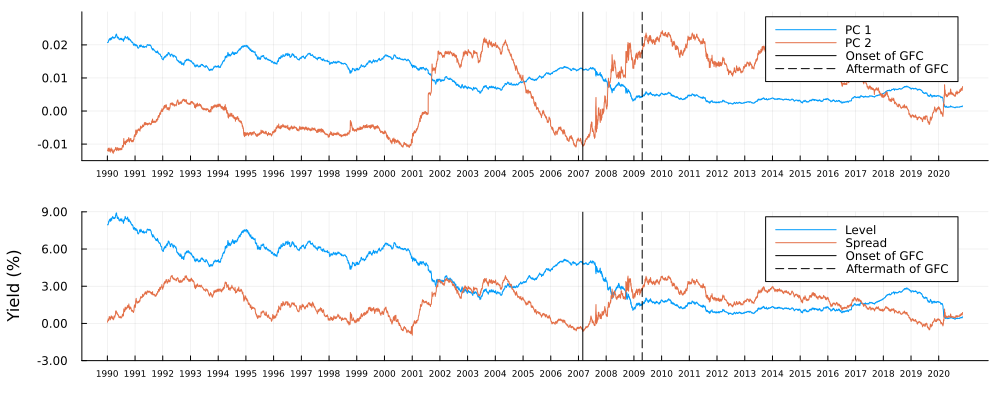
\includegraphics[width=1.0\textwidth]{results/figures/pca.png}

}

\caption{\label{fig-pca}Comparison of latent embeddings and observed
data of the US Treasury yield curve.}

\end{figure*}%

Not convinced? Let us use
\(\mathbf{Y}=\mathbf{U}\Sigma\mathbf{V}^{\prime}\) in true autoencoder
fashion to reconstruct yield curves from principal components. Let
\(z_1\) denote the first principal component and consider the following:
we keep all other \(M-1\) principal components fixed at zero where \(M\)
denotes the total number of maturities; next we traverse the latent
space by varying the value of \(z_1\) over a fixed grid of length \(K\)
each time storing the full vector \(\mathbf{z}\); finally, we vertically
concatenate the vectors and end up with a matrix \(\mathbf{Z}\) of
dimension \((K \times M)\). To reconstruct yields, we simply multiply
\(Z\) by the singular values and right singular vectors:
\(\mathbf{Y}=\mathbf{Z}\Sigma\mathbf{V}^{\prime}\).

\subsection{Example: Autoencoder}\label{example-deep-learning}

So far we have considered simple matrix decomposition. You might argue
that principal components are not really latent embeddings in the
traditional sense of deep learning. To address this, let us now consider
a simple deep-learning example. Our goal will be to not only predict
economic growth from the yield curve but also extract meaningful
features at the same time. In particular, we will use a neural network
architecture that allows us to recover a compressed latent
representation of the yield curve.

\subsubsection{Data}\label{data}

To estimate economic growth we will rely on a quarterly
\href{https://fred.stlouisfed.org/series/GDPC1}{series} of the real
gross domestic product (GDP) provided by the Federal Reserve Bank of
St.~Louis. The data arrives in terms of levels of real GDP. In order to
estimate growth, we will transform the data into log differences. Since
our yield curve data is daily, we will need to aggregate it to the
quarterly frequency. To do this, we will simply take the average of the
daily yields for each maturity. We will also standardize yields since
deep learning models tend to perform better with standardized data.
Since COVID-19 was a huge structural break, we will also filter out all
observations after 2018.

\subsubsection{Model}\label{model}

Let \(G_t\) denote growth and \(\mathbf{Y}_t\) denote the yield curve at
time \(t\). Then we are interested in a model for \(G_t\) conditional on
\(\mathbf{Y}_t\). Let \(\theta\) denote our model parameters then
formally we are interested in maximizing the likelihood
\(p_{\theta}(G_t|\mathbf{Y}_t)\). 

To do this, we will use a simple
autoencoder architecture: the encoder will consist of a single fully
connected hidden layer with 32 neurons and a hyperbolic tangent
activation function. The bottleneck layer connecting the encoder to the
decoder is a fully connected layer with 6 neurons. This is the
compressed latent representation of the yield curve mentioned above. The
decoder will consist of two fully connected layers each with a
hyperbolic tangent activation function: the first layer will consist of
32 neurons and the second layer will have the same dimension as the
input data. The output layer will consist of a single neuron with a
linear activation function. The model will be trained using the mean
squared error loss function and the Adam optimizer.

\subsubsection{Linear Probe}\label{linear-probe}

The results are shown in Figure~\ref{fig-dl-results}. The top panel
shows the actual GDP growth and fitted values from the autoencoder
model. We observe that the model captures the relationship between
economic growth and the yield curve reasonably well. As discussed above,
we also know that the relationship between economic growth and the yield
curve is characterized by two main factors: the level and the spread.
Since the model itself is fully characterized by its parameters, we
would expect that these two important factors are reflected somewhere in
the latent parameter space.

The bottleneck layer seems like a good place to start looking. To get
the latent embeddings \(\mathbf{A}_t\) at time \(t\), we simply pass the
yield curve data \(\mathbf{Y}_t\) through the encoder. Next, we follow
\cite{gurnee2023language} and use a linear probe to regress the observed
yield curve factors on the latent embeddings. Let \(F_t\) denote the
vector containing the two factors of interest in time \(t\):
\(f_t^{\text{spread}}\) and \(f_t^{\text{level}}\). Formally, we are
interested in the following regression model:
\(p_{w}(F_t|\mathbf{A}_t)\) where \(w\) denotes the regression
parameters. Following \cite{gurnee2023language}, we use Ridge regression
with \(\lambda\) set to \(0.1\). Using the estimated regression
parameters \(\hat{w}\) we can then predict the yield curve factors from
the latent embeddings: \(\hat{F}_t=\hat{w}^{\prime}\mathbf{A}_t\).

The results of this experiment are shown in the bottom panel of
Figure~\ref{fig-dl-results}. Solid lines show the observed yield curve
factors over time, while dashed lines show predicted values. We find
that the latent embeddings predict the two yield curve factors
reasonably well, in particular the spread. To put this in true
hype-lingo:

\begin{quote}
Not just a parrot! Our autoencoder neural network has an implicit
understanding of the yield curve factors and their relationship with
economic growth. It's sentient indeed!
\end{quote}

\begin{figure*}

\centering{

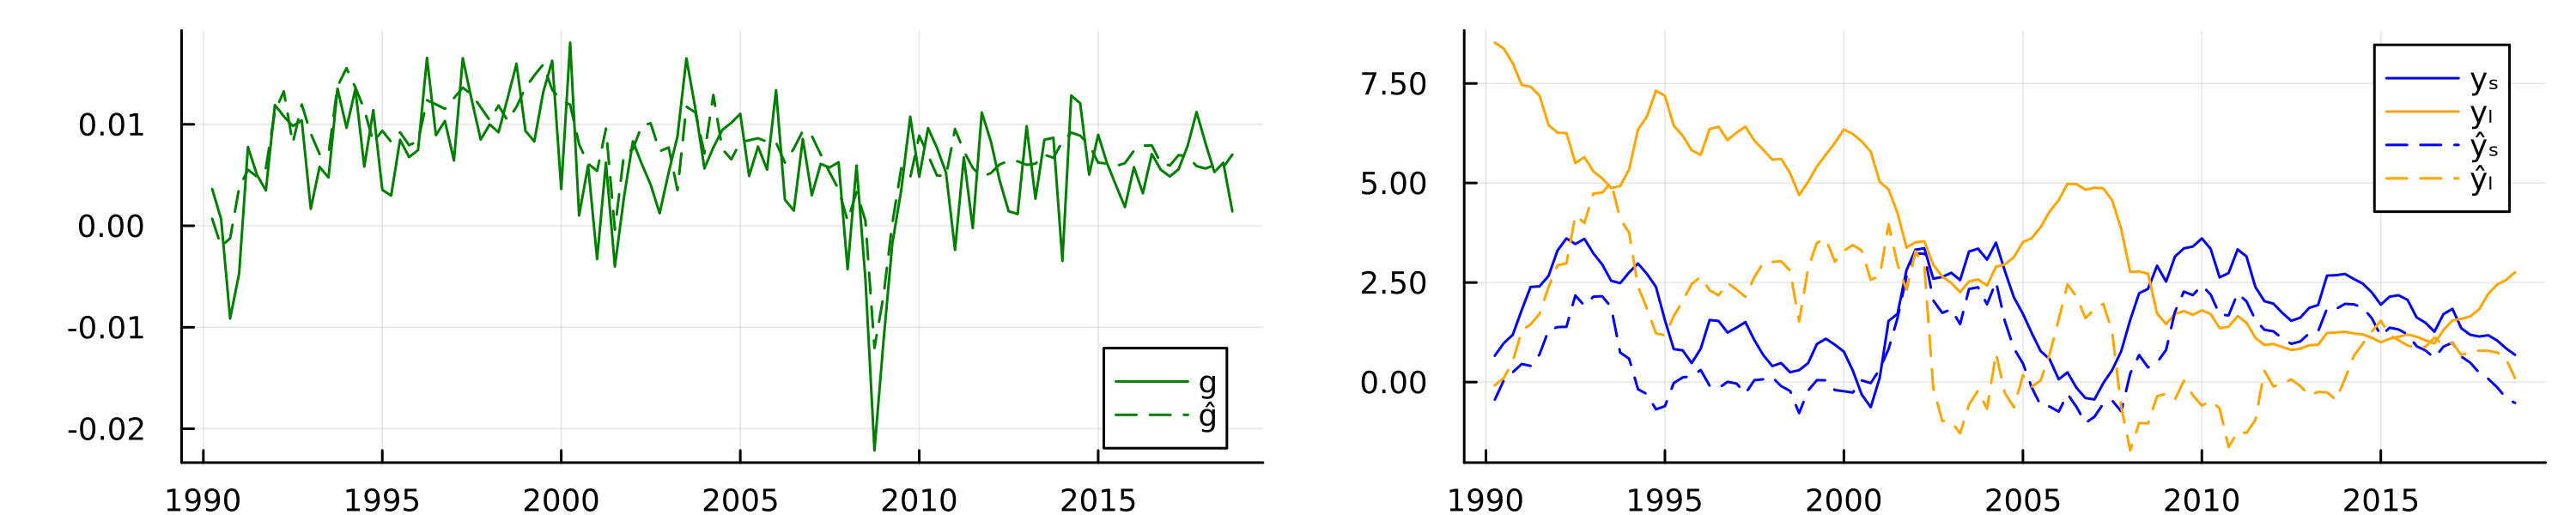
\includegraphics[width=1.0\textwidth]{results/figures/dl.png}

}

\caption{\label{fig-dl-results}The left chart shows the actual GDP growth
and fitted values from the autoencoder model. The right chart shows the
observed average level and spread of the yield curve (solid) along with
the predicted values (in-sample) from the linear probe based on the latent embeddings
(dashed).}

\end{figure*}%

\subsubsection{Ok, but truly what's the
point?}\label{ok-but-truly-whats-the-point}

The finding is not surprising but it is still interesting. In the
context of mechanistic interpretability, it demonstrates that the
black-box model has evidently learned plausible explanations for the
data. Beyond that, in this particular example, the patterns in the
latent space that we have just uncovered might actually be useful for
downstream tasks. An interesting idea could be to use the latent
embeddings as features in a more traditional and interpretable
econometric model. To demonstrate this, let us consider a simple linear
regression model for GDP growth. We will compare the performance of the
following models: (1) regressing growth \(G_t\) on the latent embedding
\(A_t\), (2) regression growth on the best subset of latent embeddings
\(A_t\), (3) regressing growth on lagged growth, (4) regressing growth
on lagged growth and the observed yield curve factors \(F_t\), (5)
regressing growth on the best subset of yield curve factors \(F_t\),
and, finally, (5) regressing growth on lagged growth and the best subset
of latent embeddings \(A_t\).

The results are shown in the table below. The key finding of interest is
that the coefficients on the latent embeddings in model (5) are
statistically significant. This suggests that the latent embeddings
contain information that is useful for predicting GDP growth.

\begin{tabular}{lrr}
\toprule
              &  \multicolumn{2}{c}{GDP Growth} \\ 
\cmidrule(lr){2-3} 
              &            (1) &            (2) \\ 
\midrule
(Intercept)   &          0.002 &       0.004*** \\ 
              &        (0.002) &        (0.001) \\ 
Lagged Growth &       0.385*** &       0.344*** \\ 
              &        (0.089) &        (0.088) \\ 
Spread        &          0.000 &                \\ 
              &        (0.001) &                \\ 
Level         &          0.000 &                \\ 
              &        (0.000) &                \\ 
Embedding 6   &                &         0.008* \\ 
              &                &        (0.003) \\ 
\midrule
Obs.          &            114 &            114 \\ 
BIC           &       -857.429 &       -864.499 \\ 
R²            &          0.168 &          0.203 \\ 
\bottomrule
\end{tabular}


\subsection{Example: Large Language Model}\label{ex-llm}

To round up this section, we will jump back on the hype train and
consider an example involving an LLM. In particular, we will closely
follow the approach in \cite{gurnee2023language} and apply it to a novel
financial dataset: the \emph{Trillion Dollar Words} dataset introduced
by \cite{shah2023trillion}. The dataset contains a curated
selection of sentences formulated by central bankers of the US Federal
Reserve and communicated to the public in speeches, meeting minutes and
press conferences. The authors of the paper use this dataset to train
LLMs to classify sentences as either `dovish', `hawkish' or `neutral'.
To this end, they first manually annotate a subsample of the available
data and then fine-tune various foundation models. Their model of
choice, \emph{FOMC-RoBERTa} (a fine-tuned version of RoBERTa \cite{liu2019roberta}), achieves an \(F_1\) score of around \(>0.7\) for the
classification task. To illustrate the potential usefulness of the
learned classifier, they use predicted labels for the entire dataset to
compute an ad-hoc, count-based measure of `hawkishness'. They then go on
to show that this measure correlates with key economic indicators in the
expected direction: when inflationary pressures rise, the measured level
of `hawkishness' increases as central bankers need to raise interest
rates to bring inflation back to target.

\subsubsection{Linear Probes}\label{linear-probes}

Instead of computing a measure based on predicted labels, we can use linear probes to assess if the fine-tuned model has learned associative patterns between central bank communications and key economic indicators. To this end, we have further pre-processed the data provided by \cite{shah2023trillion} and used their proposed model to compute layer-wise embeddings for all available sentences. We have made these available and easily accessible through a small Julia package: \href{https://anonymous.4open.science/r/TrillionDollarWords/README.md}{TrillionDollarWords.jl}. For each layer, we have then computed linear probes on two inflation indicators---the Consumer Price Index (CPI) and the Producer Price Index (PPI)---as well as US Treasury yields at different levels of maturity. 

To mitigate issues related to over-parameterization, we follow the recommendation in \cite{alain2018understanding} to first reduce the dimensionality of the embeddings each time. In particular, linear probes are restricted to the first 128 principal components of the embeddings
of each layer.

Figure~\ref{fig-fomc} highlights the result for the linear probe
on the CPI. The chart shows various performance measures plotted against
\emph{FOMC-RoBERTa}'s \(n\)-th layer. Shaded areas show the variation
across cross-validation folds, where we have used an expanding window
approach to split the time series. To avoid look-ahead bias, we run PCA
separately for each training set. Results for the linear probes are
shown along with results for autoregressive models (AR) used as our
baseline.

The first column shows the correlations between model predictions and
observed inflation. One can observe that this correlation is strictly
positive for the baseline models and the linear probes. Consistent with
the findings in \cite{gurnee2023language} and \cite{alain2018understanding},
we also observe that this correlation tends to be higher for layers near
the end of the transformer model. Those layers produce predictions that
are more positively correlated with observed inflation than those
produced by the corresponding autoregressive models.

Similarly, we observe that the (root) mean squared error of the linear
probe is largely on par with the baseline. The average prediction error
is gradually reduced as we move along the horizontal axis, which is
again indicative of the notion that layers closer to the end of the
neural network have distilled more useful representations.

\begin{figure*}

\centering{

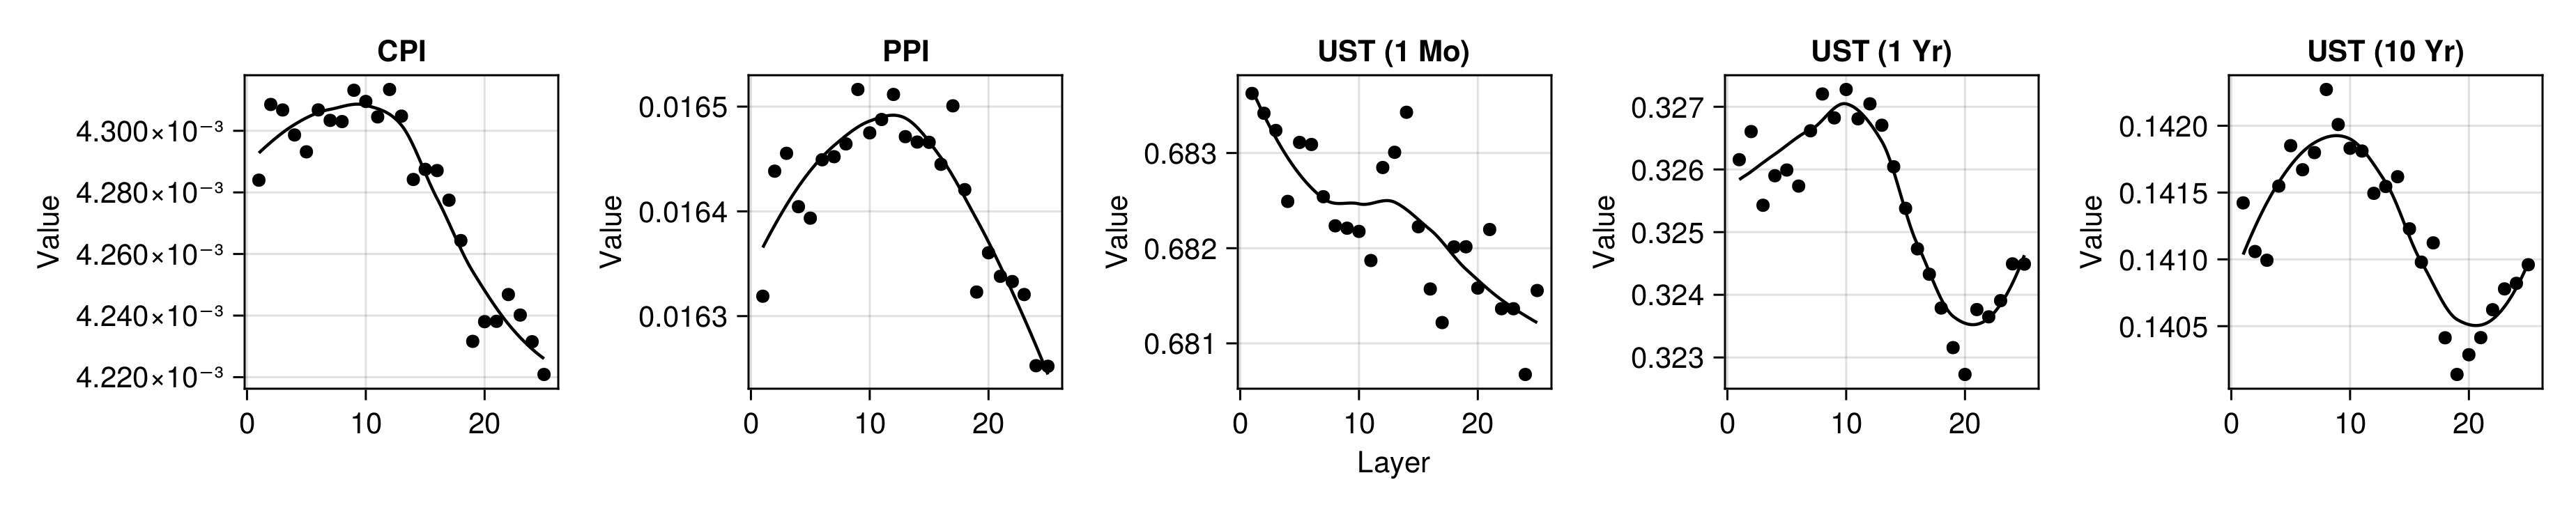
\includegraphics[width=1.0\textwidth]{results/figures/rmse_pca_128.png}

}

\caption{\label{fig-fomc}Various performance measures (correlation and
(root) mean squared error) plotted against \emph{FOMC-RoBERTa}'s
\(n\)-th layer. Shaded areas indicate variation across cross-validation
folds, where we have used an expanding window approach to split the time
series. Results for the linear probes are shown along with results for
autoregressive models (AR). The optimal lag length was determined using
the Bayes Information Criterium.}

\end{figure*}%

\begin{figure*}

\centering{

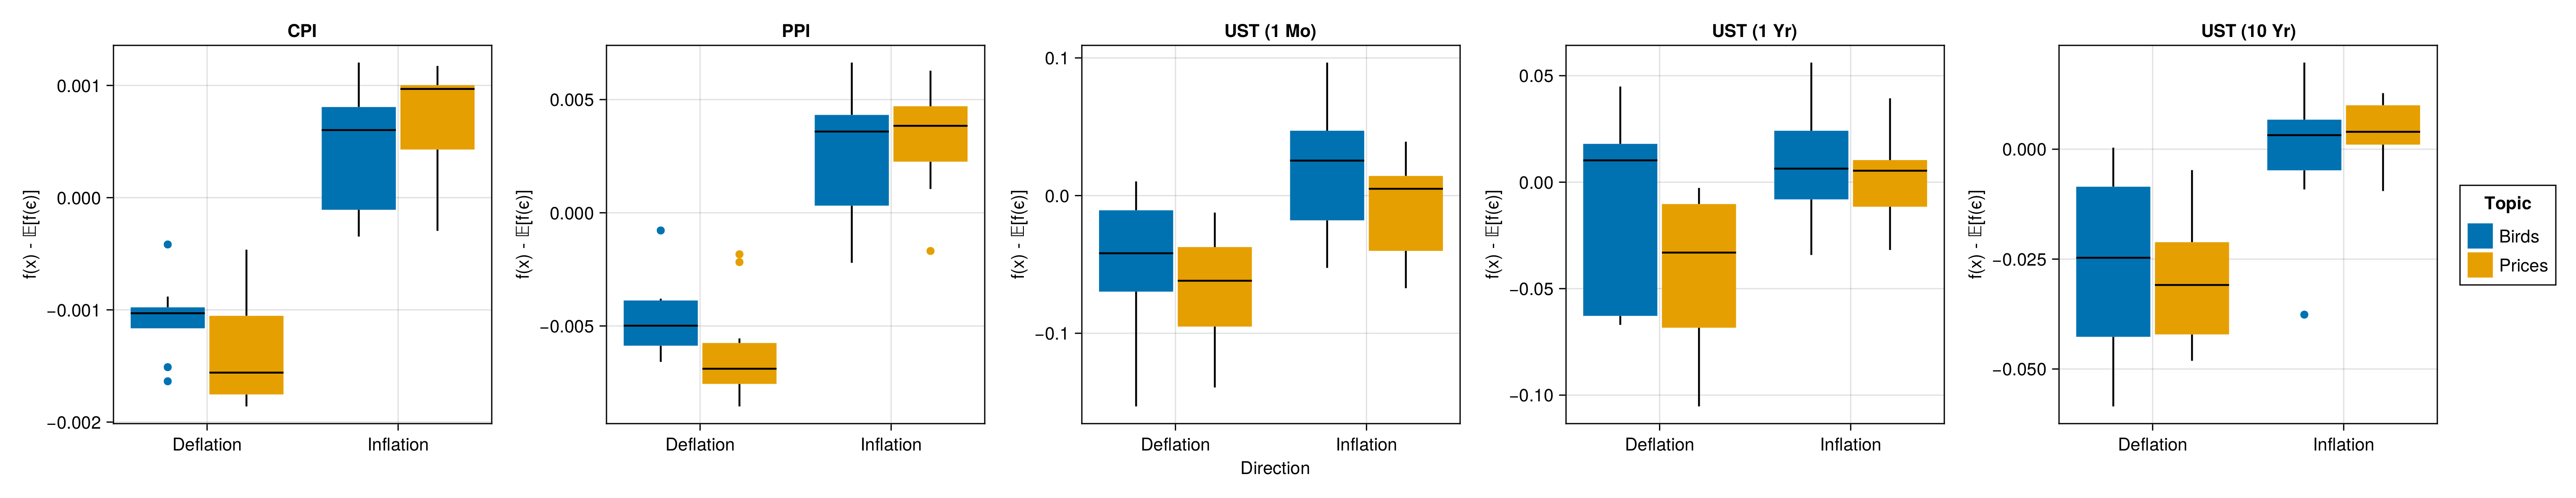
\includegraphics[width=1.0\textwidth]{results/figures/attack_all_measures.png}

}

\caption{\label{fig-attack}Probe predictions for sentences about
inflation of prices (IP), deflation of prices (DP), inflation of birds
(IB) and deflation of birds (DB). The vertical axis shows predicted
inflation levels subtracted by the average predicted inflation level for
the whole sample period (train and test set).}

\end{figure*}%

\subsubsection{Stochastic Parrots After
All?}\label{stochastic-parrots-after-all}

These results from the linear probe shown in Figure~\ref{fig-fomc} are
certainly not unimpressive: even though \emph{FOMC-RoBERTa} was not
explicitly trained to uncover associations between central bank
communications and the level of consumer prices, it appears that the
model has distilled representations that can be used to predict
inflation. It is worth pointing out here that this model is
substantially smaller than the models tested in \cite{gurnee2023language}. This begs the following question:

\begin{quote}
Have we uncovered further evidence that LLMs ``aren't mere stochastic
parrots''? Has \emph{FOMC-RoBERTa} developed an intrinsic understanding
of the economy just by `reading' central bank communications?
\end{quote}

We are having a very hard time believing this. To argue our case, we will now produce a counter-example demonstrating that, if anything, these findings are very much in line with the parrot metaphor. The counter example is based on the following premise: if the results from the linear probe truly were indicative of some intrinsic understanding of the economy, then the probe should not be sensitive to random sentences  that are most definitely not related to consumer prices.

To test this, we select the best-performing probe trained on the final-layer activations to predict changes in the CPI. We then make up sentences that fall into one of these four categories: \emph{Inflation/Prices} (IP)---sentences about price inflation, \emph{Deflation/Prices} (DP)---sentences about price deflation, \emph{Inflation/Birds} (IB)---sentences about an inflation in the number of birds and \emph{Deflation/Birds} (DB)---sentences about a deflation in the number of birds. A sensible sentence for category DP, for example, could be: ``It is essential to bring inflation back to target to avoid drifting into deflation territory.''. Analogically, we could construct the following sentence for the DB category: ``It is essential to bring the numbers of doves back to target to avoid drifting into dovelation territory.''.

In light of the encouraging results for the probe in
Figure~\ref{fig-fomc}, we should expect the probe to predict higher
levels of inflation for activations for sentences in the IP category
than for sentences in the DP category. If this was indicative of true
intrinsic understanding, we would not expect to see any significant
difference in predicted inflation levels for sentences about birds,
independent of whether or not their numbers are increasing. More
specifically, we would not expect the probe to predict values for
sentences about birds that are substantially different from the values
it can be expected to predict when using actual white noise as inputs.

To get to this last point, we also generate many probe predictions for
samples of noise. Let \(f: \mathcal{A}^k \mapsto \mathcal{Y}\) denote
the linear probe that maps from the \(k\)-dimensional space spanned by
\(k\) first principal components of the final-layer activations to the
output variable of interest (CPI growth in this case). Then we sample
\(\varepsilon_i \sim \mathcal{N}(\mathbf{0},\mathbf{I}^{(k \times k)})\)
for \(i \in [1,1000]\) and compute the sample average. We repeat this
process \(10000\) times and compute the median-of-means to get an
estimate for \(\mathbb{E}[f(\varepsilon)]=\mathbb{E}[y|\varepsilon]\),
that is the predicted value of the probe conditional on white noise.

Next, we propose the following hypothesis test as a minimum viable
testing framework to assess if the probe results (may) provide evidence
for an actual understanding of key economic relationships learned purely
from text:

\begin{proposition}[Parrot
Test]\protect\hypertarget{prp-line}{}\label{prp-line}

~

\begin{itemize}
\tightlist
\item
  \emph{H0} (Null \emph{WEAK}): The probe never predicts values that are
  statistically significantly different from
  \(\mathbb{E}[f(\varepsilon)]\)
\item
  \emph{H1} (Stochastic Parrots \emph{RISKIER}): The probe predicts
  values that are statistically significantly different from
  \(\mathbb{E}[f(\varepsilon)]\) for sentences in all categories
  (IP,DP,IB,DB).
\item
  \emph{H2} (More than Mere Stochastic Parrots \emph{RISKIEST}): The
  probe predicts values that are statistically significantly different
  from \(\mathbb{E}[f(\varepsilon)]\) for sentences in categories IP and
  DP, but not for sentences in IB and DB.
\end{itemize}

\end{proposition}

To be clear, if in such a test we did find substantial evidence in
favour of rejecting both \emph{HO} and \emph{H1}, this would not
automatically imply that \emph{H2} is true. But to even continue
investigating if based on having learned meaningful representation the
underlying LLM is more than just a parrot, it should be able to pass
this simple test.

In this particular case, Figure~\ref{fig-attack} demonstrates that we
find some evidence to reject \emph{H0} but not \emph{H1} for
\emph{FOMC-RoBERTa}. The median linear probe predictions for sentences
about inflation and deflation are indeed substantially higher and lower,
respectively than for random noise. Unfortunately, the same is true for
sentences about the inflation and deflation in the number of birds,
albeit to a somewhat lower degree.

We should note that the number of sentences in each category is very
small here (10), so the results in Figure~\ref{fig-attack} cannot be
used to establish statistical significance. That being said, even a
handful of convincing counter-examples should be enough for us to
seriously question the claim that results from linear probes provide
evidence against the parrot metaphor. In fact, if there's even a single
sentence for which any

\begin{quote}
Strong alternative hypothesis to address own confirmation bias
Articulating a test to better differentiate
\end{quote}

\subsection{Discussion of Examples}

Our examples should not be seen as an attempt to conclusively refute claims that LLMs can develop on actual "understanding" of the world by distilling knowledge in more compact representations. We hope that they serve to illustrate, however, that the use of diagnostic tools is potentially misleading and most definitely insufficient in providing evidence in favor of "understanding". Linear probes and related tools from mechanistic interpretability were proposed in the context of monitoring models and diagnosing potential problems \citep{alain2018understanding}. Favourable outcomes from probes merely indicate that the model "has learned information relevant for the property [of interest]" \citep{belinkov2021probing}. Our examples demonstrate that this is achievable even for small models, that most readers will agree have certainly not developed an intrinsic "understanding" of the world. The fact that even these models distill meaningful representations goes to show that more conservative and rigorous tests are needed to draw conclusions about the emerging capabilities of AI models.

\bibliography{biblio}
\bibliographystyle{icml2024}


%%%%%%%%%%%%%%%%%%%%%%%%%%%%%%%%%%%%%%%%%%%%%%%%%%%%%%%%%%%%%%%%%%%%%%%%%%%%%%%
%%%%%%%%%%%%%%%%%%%%%%%%%%%%%%%%%%%%%%%%%%%%%%%%%%%%%%%%%%%%%%%%%%%%%%%%%%%%%%%
% APPENDIX
%%%%%%%%%%%%%%%%%%%%%%%%%%%%%%%%%%%%%%%%%%%%%%%%%%%%%%%%%%%%%%%%%%%%%%%%%%%%%%%
%%%%%%%%%%%%%%%%%%%%%%%%%%%%%%%%%%%%%%%%%%%%%%%%%%%%%%%%%%%%%%%%%%%%%%%%%%%%%%%
\newpage
\appendix
\onecolumn
\section{You \emph{can} have an appendix here.}

You can have as much text here as you want. The main body must be at most $8$ pages long.
For the final version, one more page can be added.
If you want, you can use an appendix like this one.  

The $\mathtt{\backslash onecolumn}$ command above can be kept in place if you prefer a one-column appendix, or can be removed if you prefer a two-column appendix.  Apart from this possible change, the style (font size, spacing, margins, page numbering, etc.) should be kept the same as the main body.
%%%%%%%%%%%%%%%%%%%%%%%%%%%%%%%%%%%%%%%%%%%%%%%%%%%%%%%%%%%%%%%%%%%%%%%%%%%%%%%
%%%%%%%%%%%%%%%%%%%%%%%%%%%%%%%%%%%%%%%%%%%%%%%%%%%%%%%%%%%%%%%%%%%%%%%%%%%%%%%


\end{document}


% This document was modified from the file originally made available by
% Pat Langley and Andrea Danyluk for ICML-2K. This version was created
% by Iain Murray in 2018, and modified by Alexandre Bouchard in
% 2019 and 2021 and by Csaba Szepesvari, Gang Niu and Sivan Sabato in 2022.
% Modified again in 2023 and 2024 by Sivan Sabato and Jonathan Scarlett.
% Previous contributors include Dan Roy, Lise Getoor and Tobias
% Scheffer, which was slightly modified from the 2010 version by
% Thorsten Joachims & Johannes Fuernkranz, slightly modified from the
% 2009 version by Kiri Wagstaff and Sam Roweis's 2008 version, which is
% slightly modified from Prasad Tadepalli's 2007 version which is a
% lightly changed version of the previous year's version by Andrew
% Moore, which was in turn edited from those of Kristian Kersting and
% Codrina Lauth. Alex Smola contributed to the algorithmic style files.
